\begin{figure}[!t]
\centering
\begin{subfigure}[t]{0.49\textwidth}
\centering
\begingroup
\setlength{\tabcolsep}{1pt}
\begin{tabular}{@{}cc@{}}
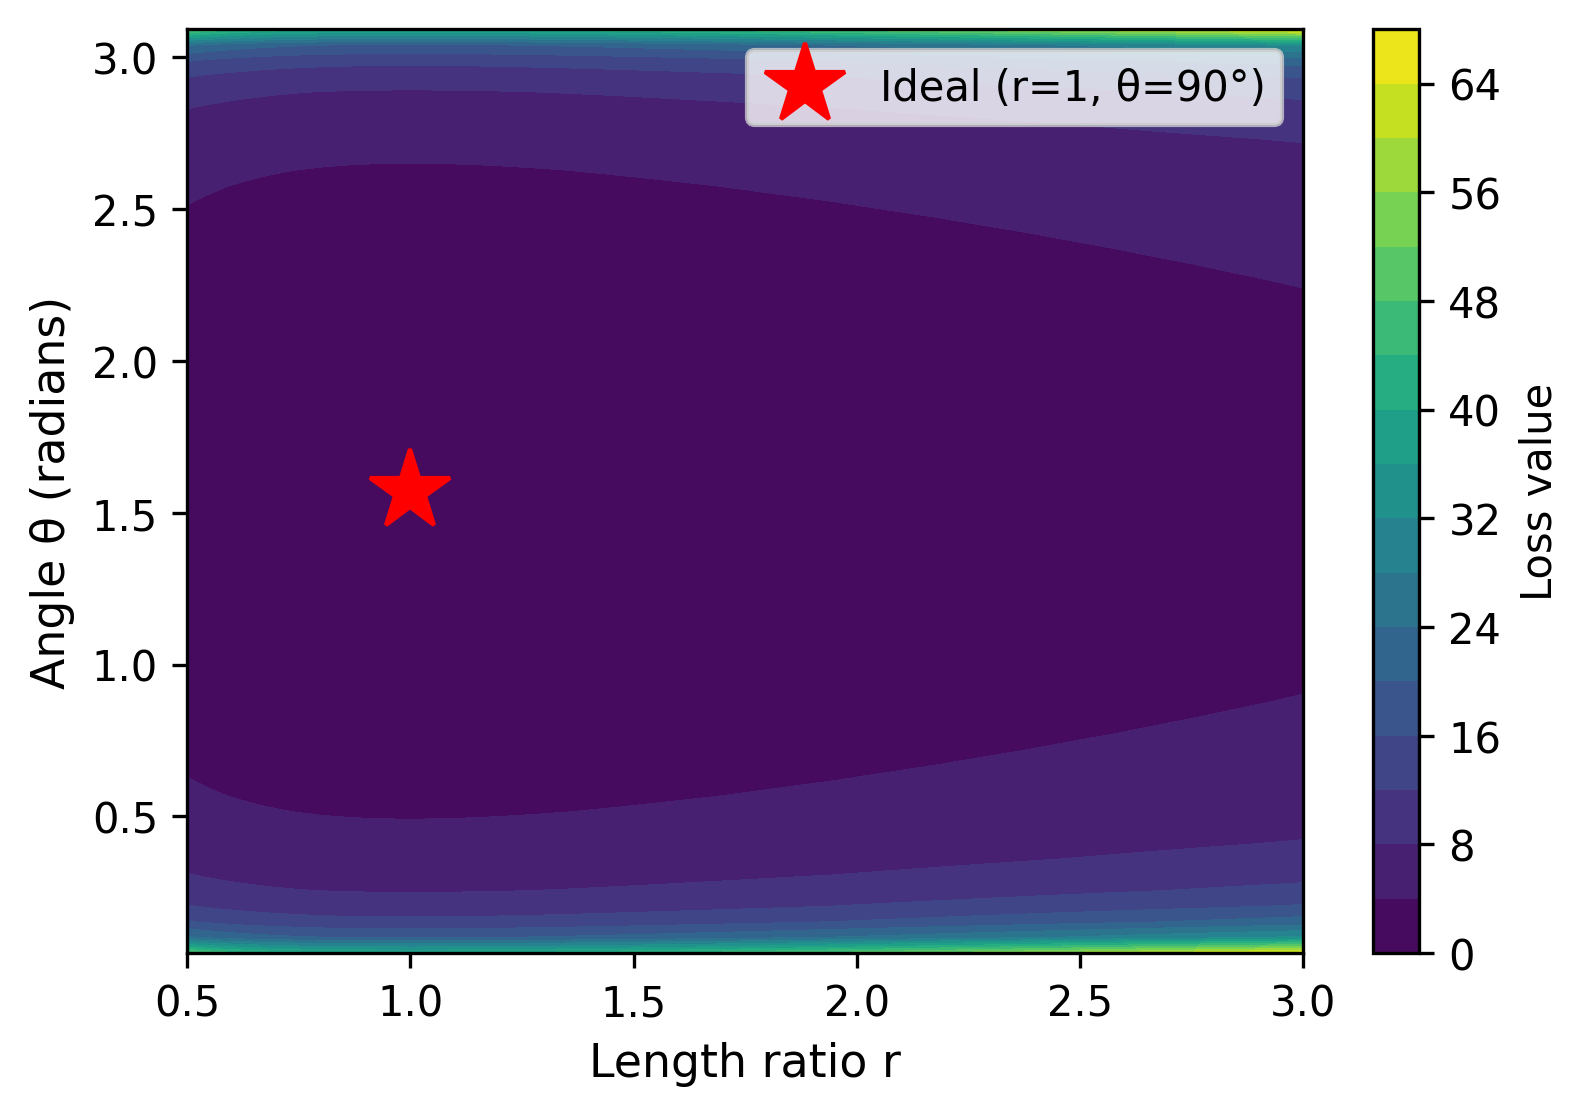
\includegraphics[width=0.48\linewidth]{../figures/loss_2d_condition_number.png} &
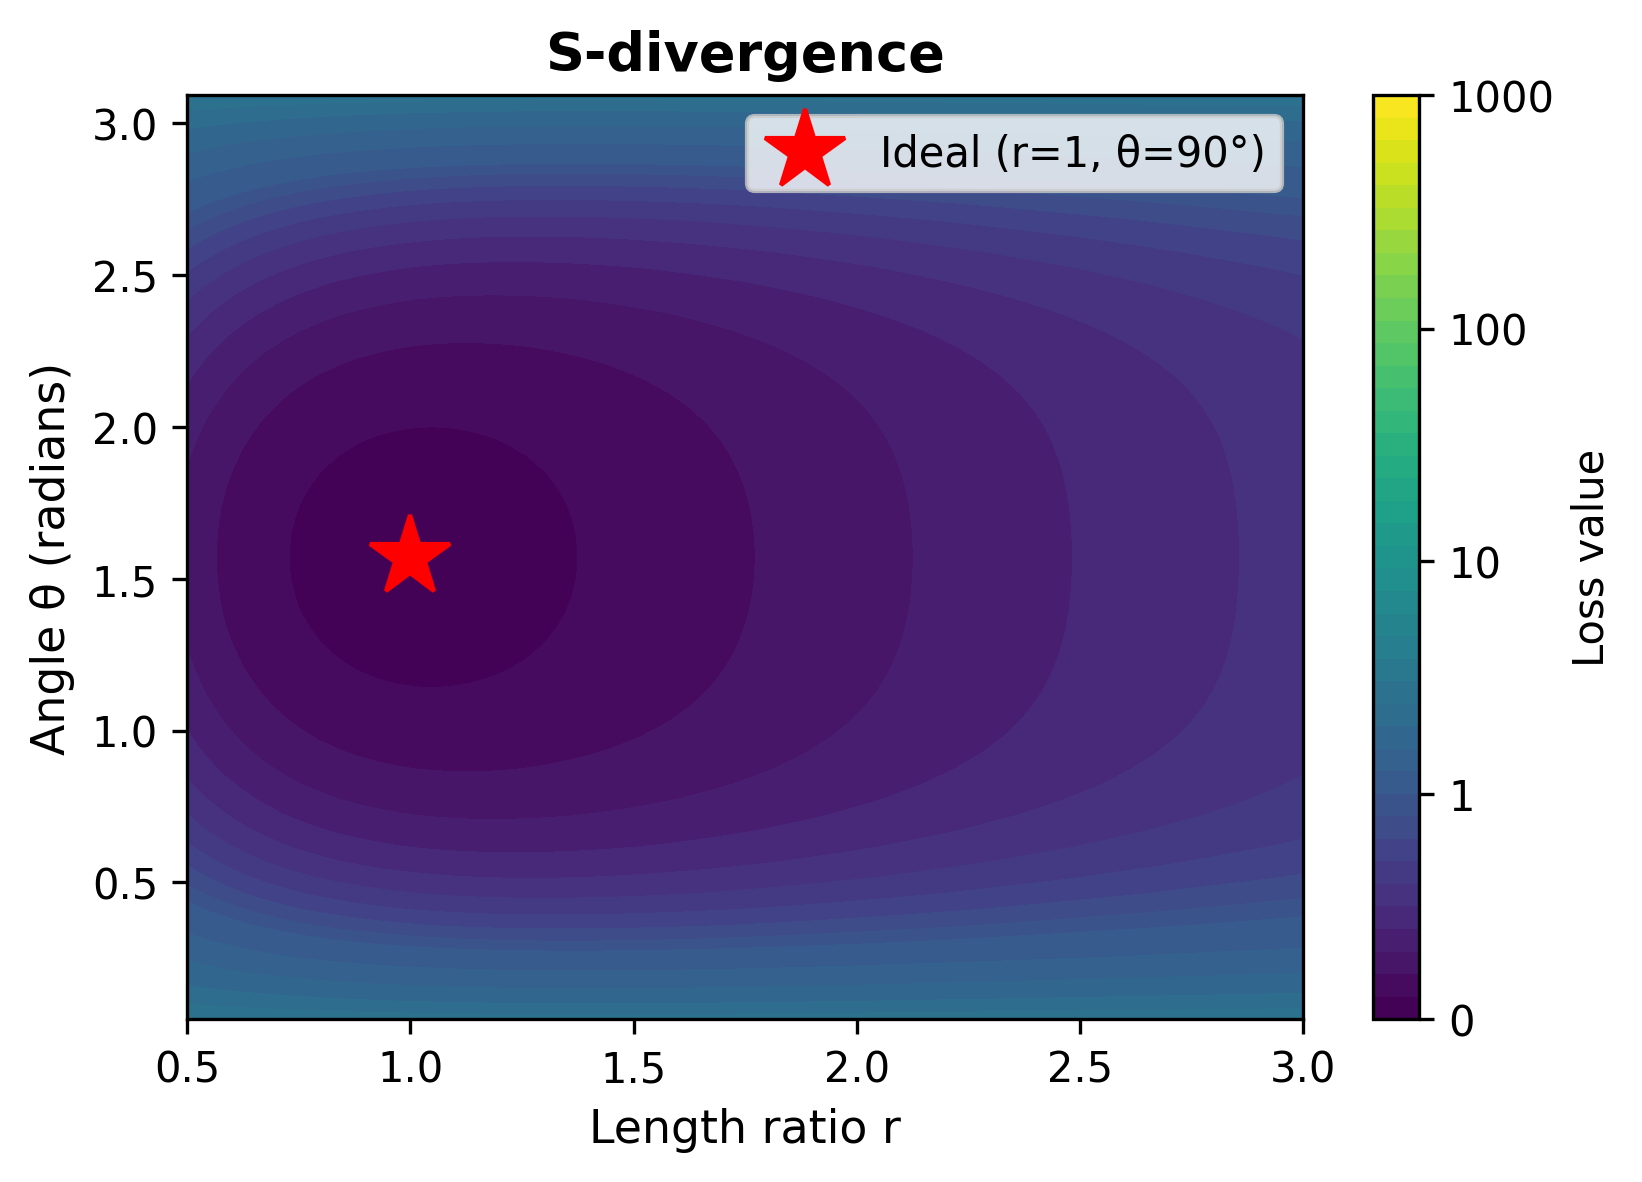
\includegraphics[width=0.48\linewidth]{../figures/loss_2d_s_divergence_identity.png} \\
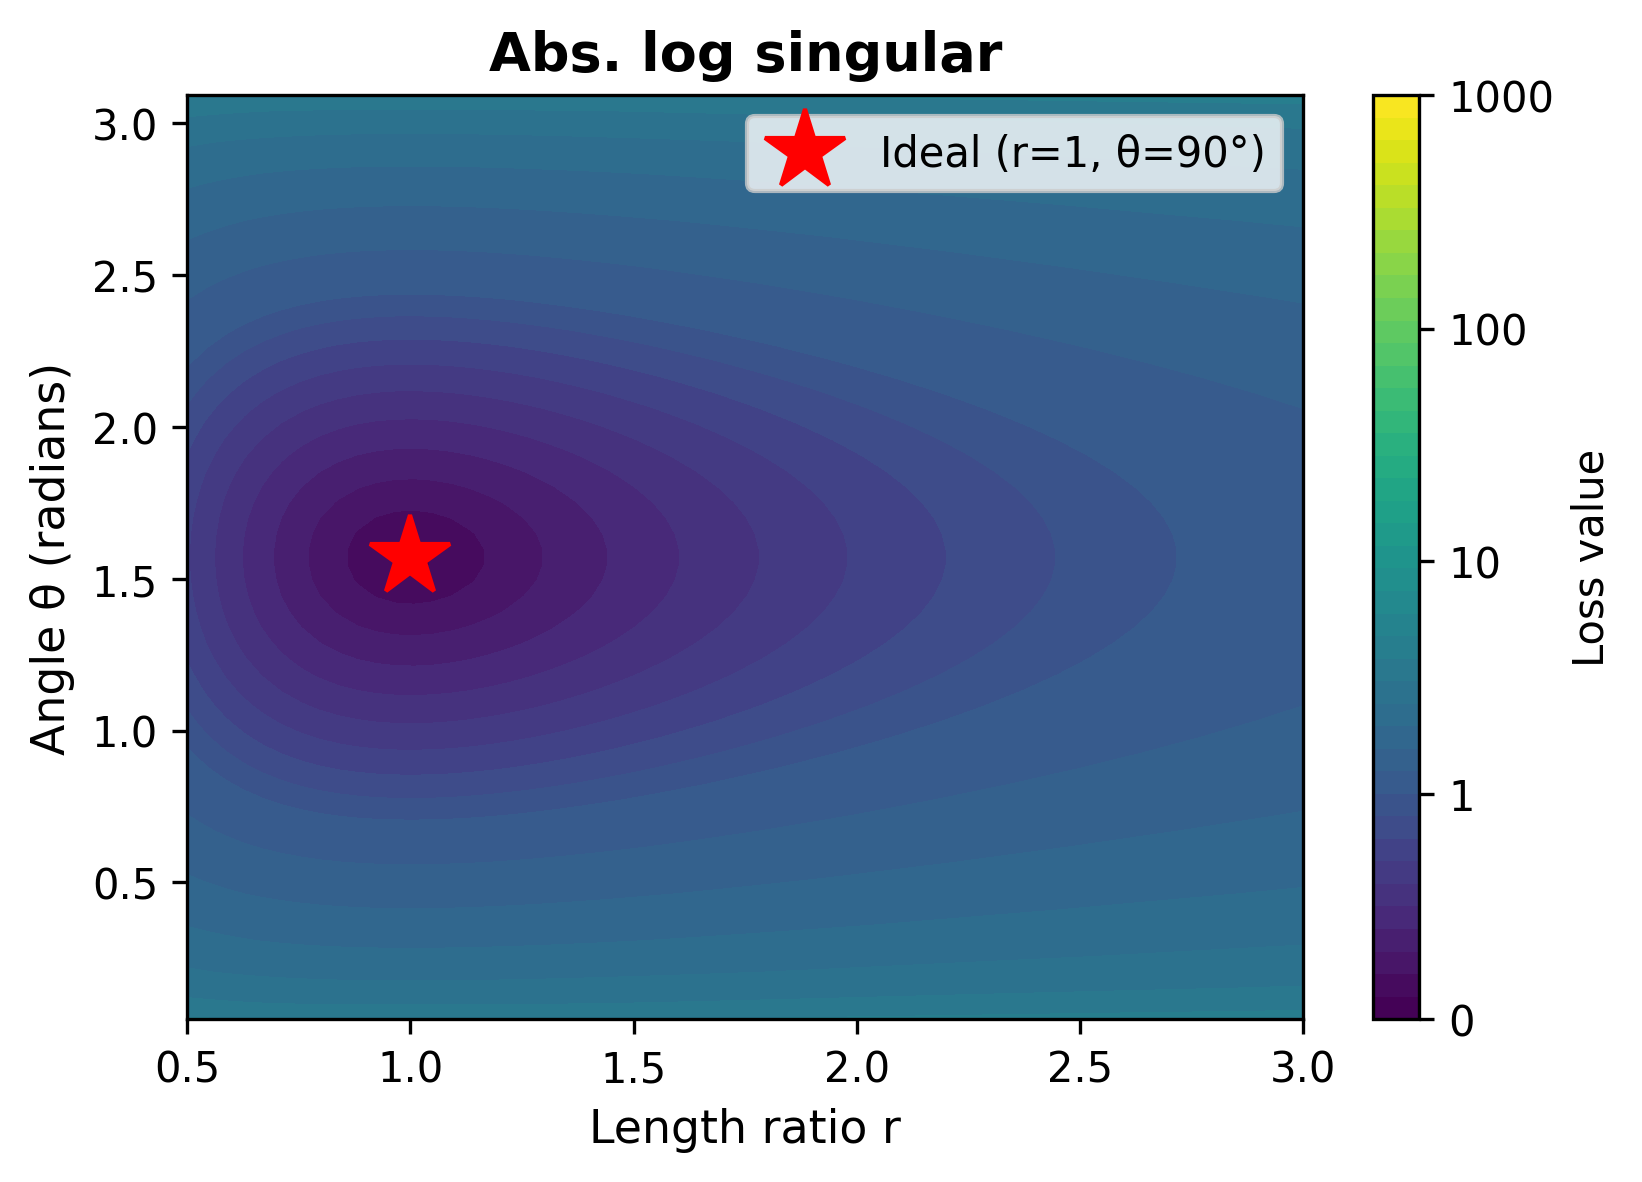
\includegraphics[width=0.48\linewidth]{../figures/loss_2d_absolute_log_singular_values.png} &
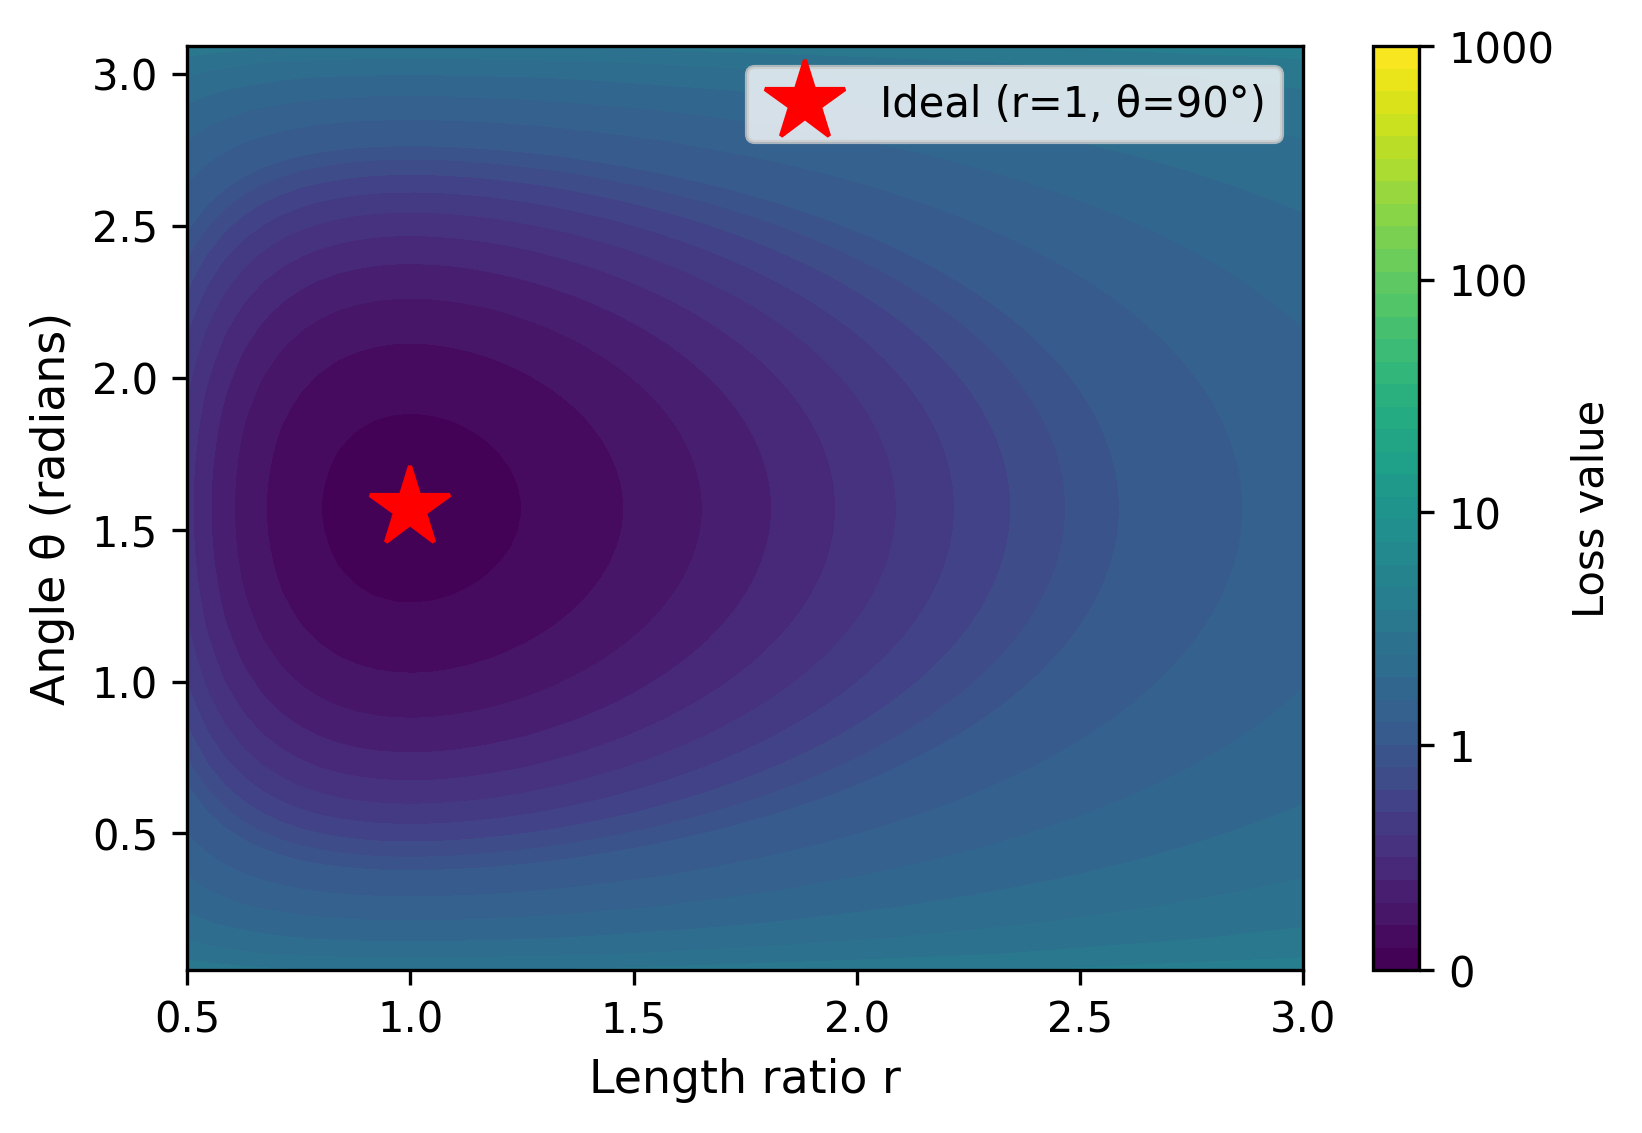
\includegraphics[width=0.48\linewidth]{../figures/loss_2d_normalized_logdet_volume.png} \\
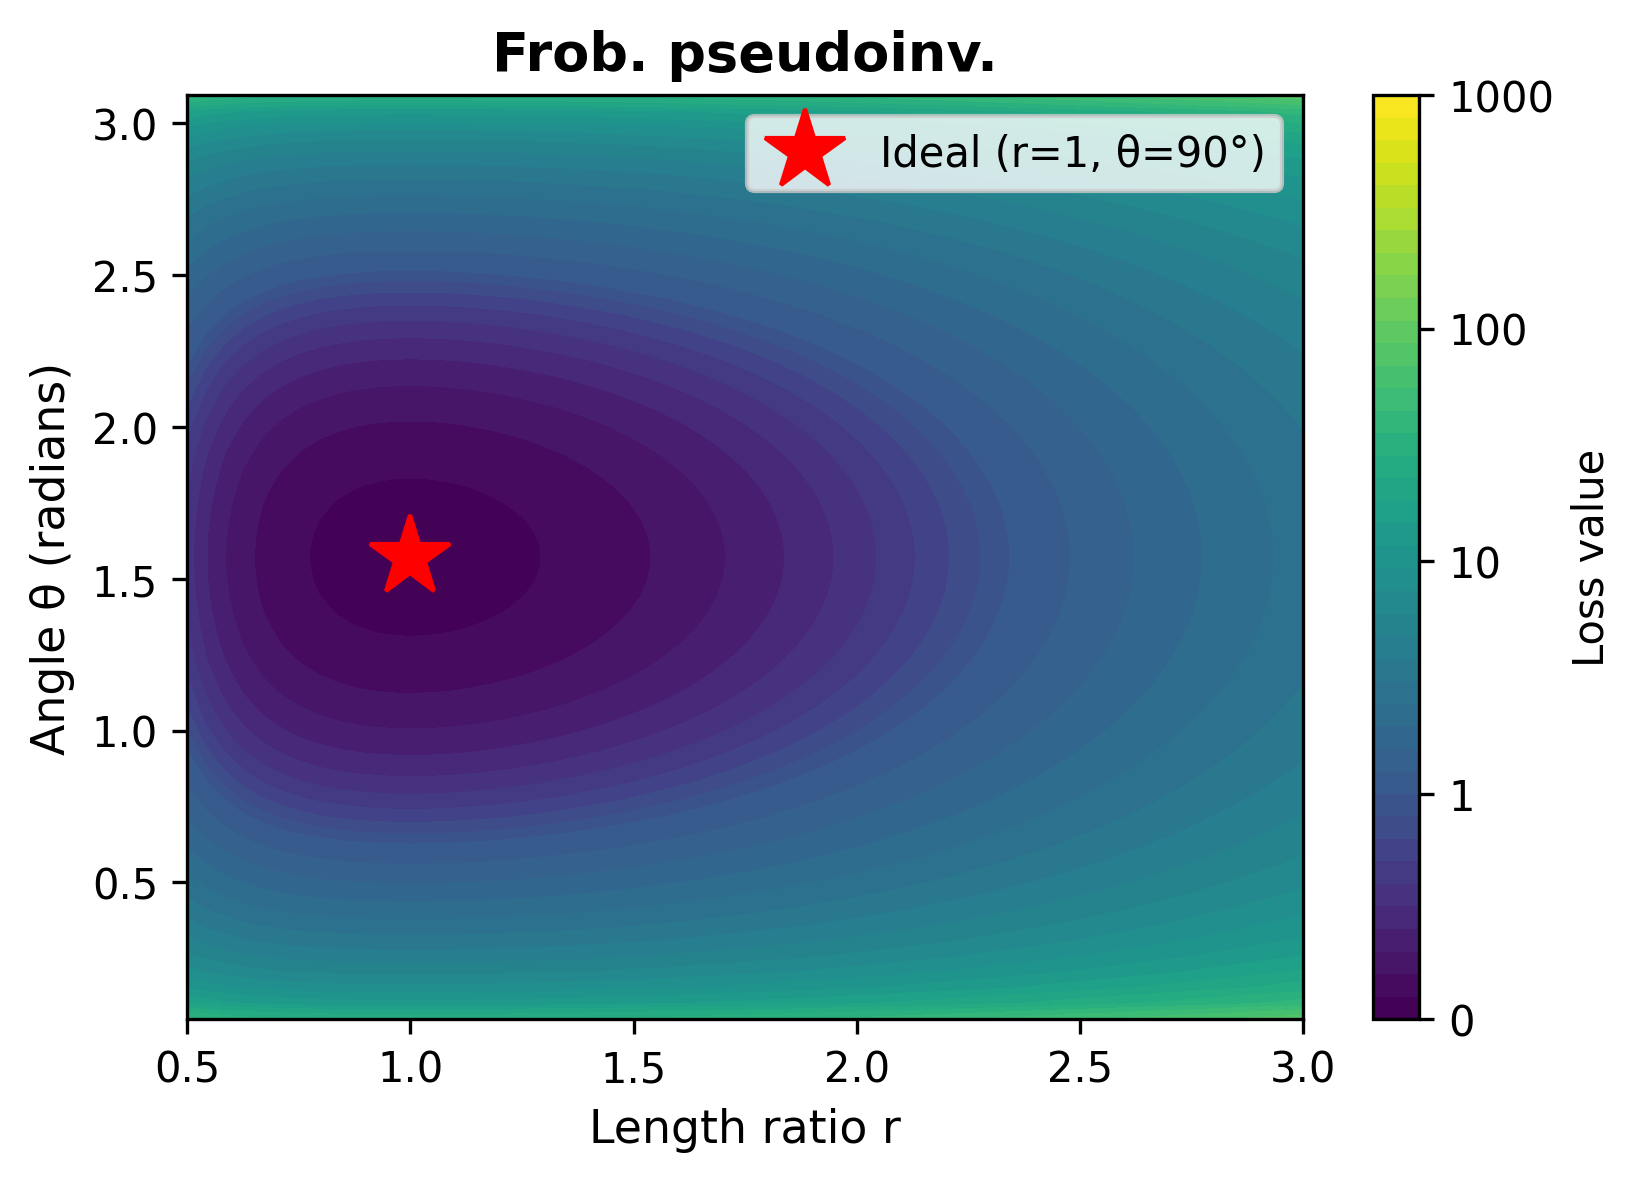
\includegraphics[width=0.48\linewidth]{../figures/loss_2d_frob_pseudoinverse.png} &
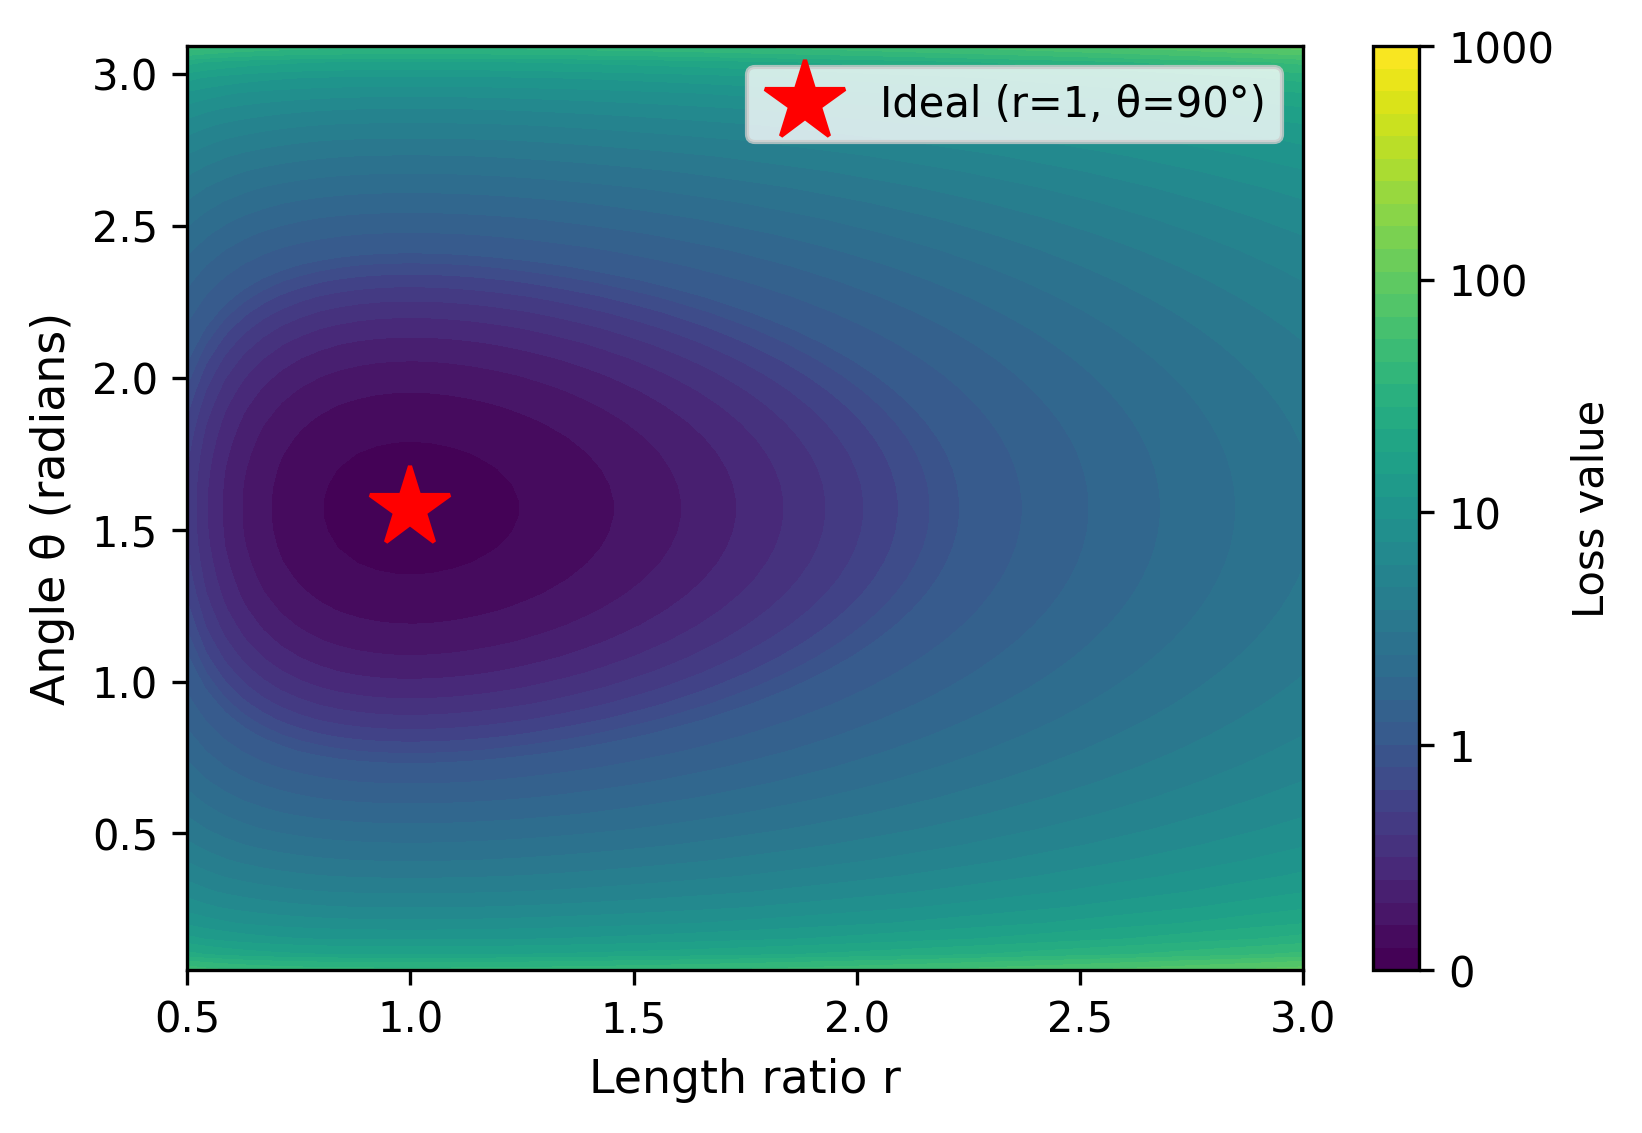
\includegraphics[width=0.48\linewidth]{../figures/loss_2d_gl_pseudoinverse.png}
\end{tabular}
\endgroup \caption{$2 \times 2$ matrices.}
\label{fig:loss_landscapes}
\end{subfigure}\hfill
\begin{subfigure}[t]{0.49\textwidth}
\centering
\begingroup
\setlength{\tabcolsep}{1pt}
\begin{tabular}{@{}cc@{}}
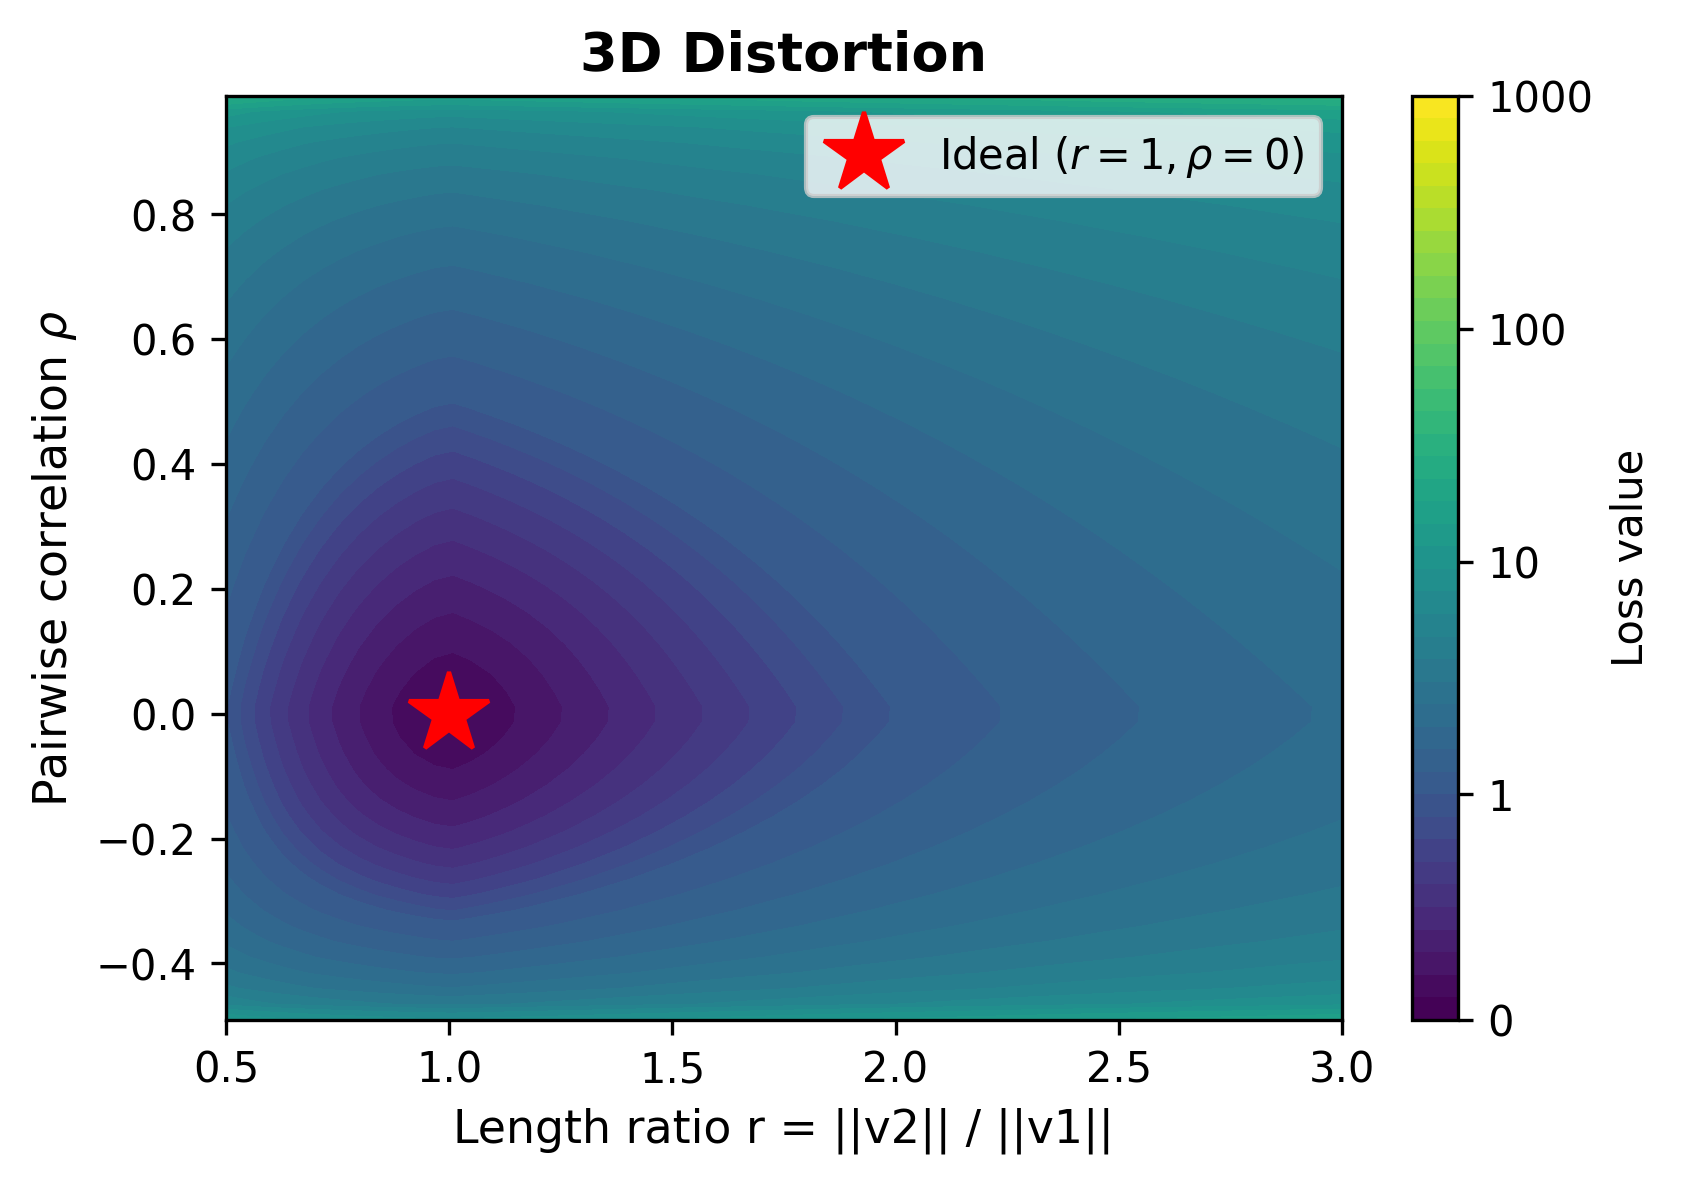
\includegraphics[width=0.48\linewidth]{../figures/loss_3d_equicorr_condition_number.png} &
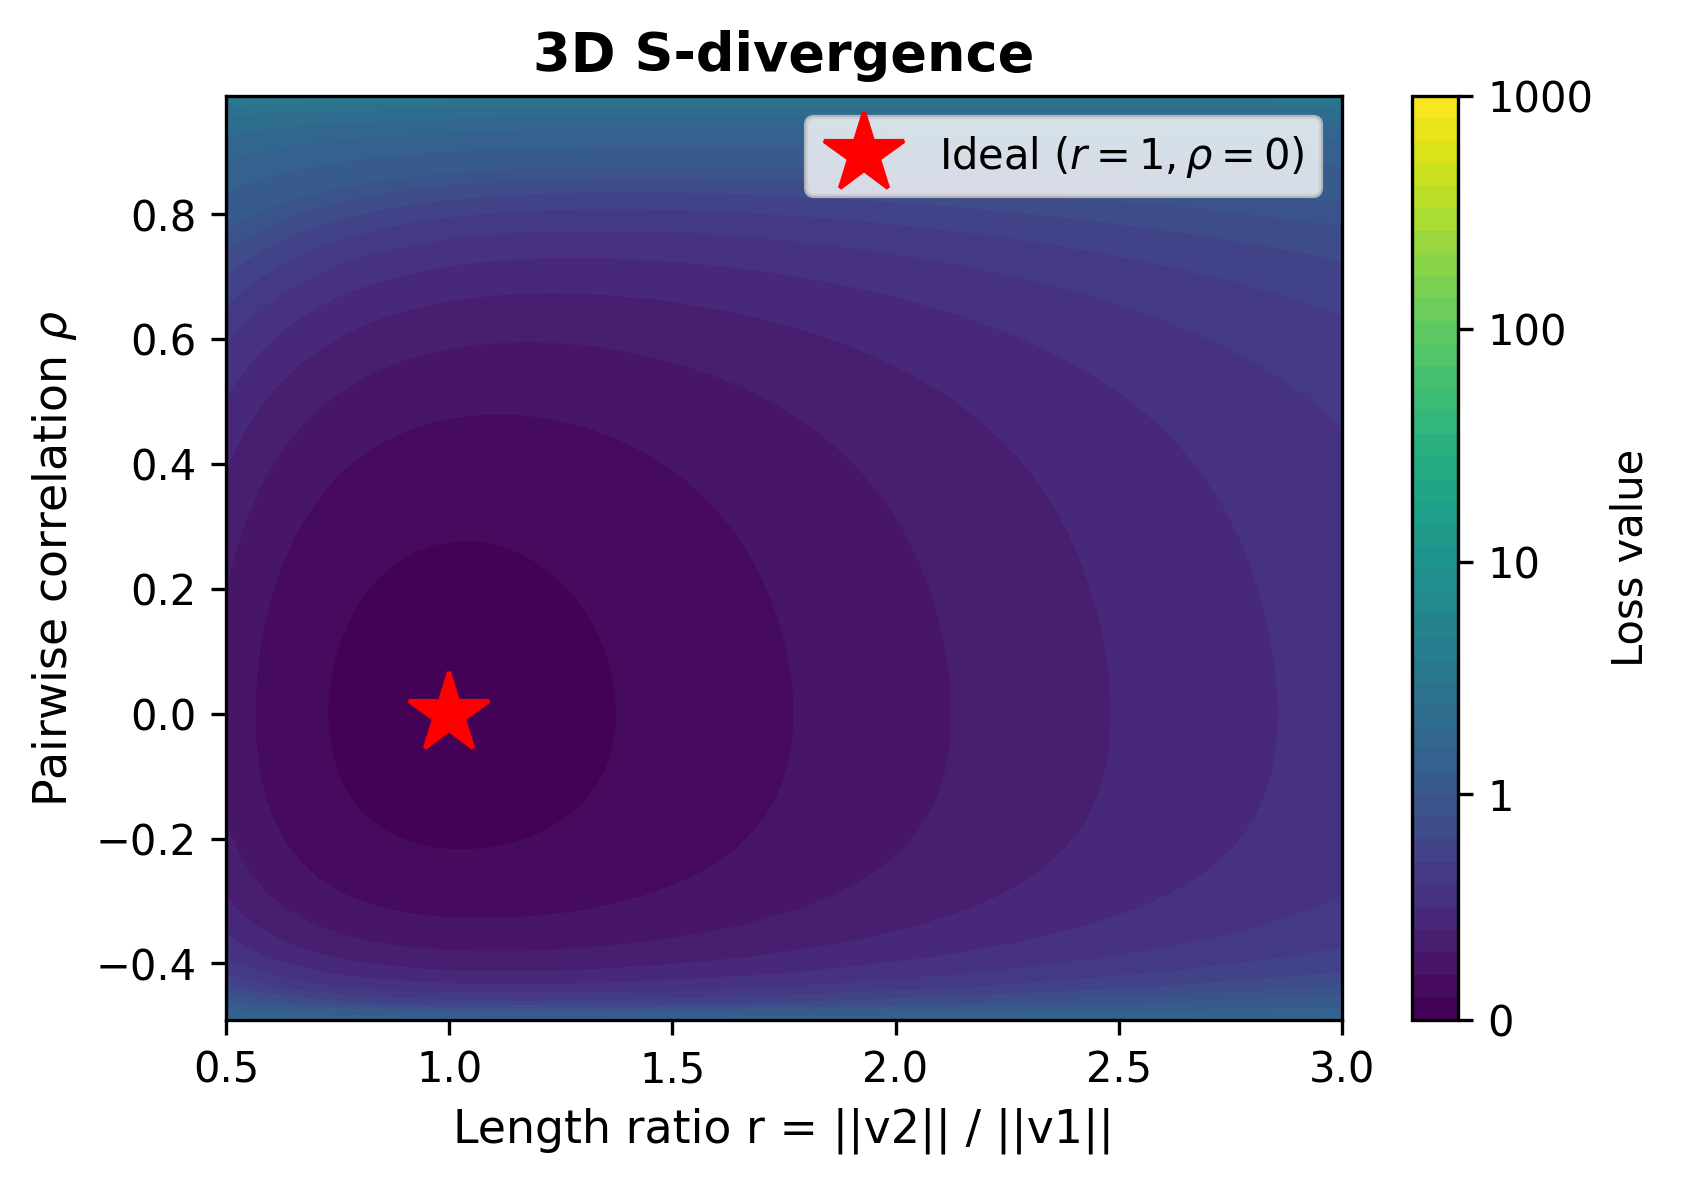
\includegraphics[width=0.48\linewidth]{../figures/loss_3d_equicorr_s_divergence_identity.png} \\
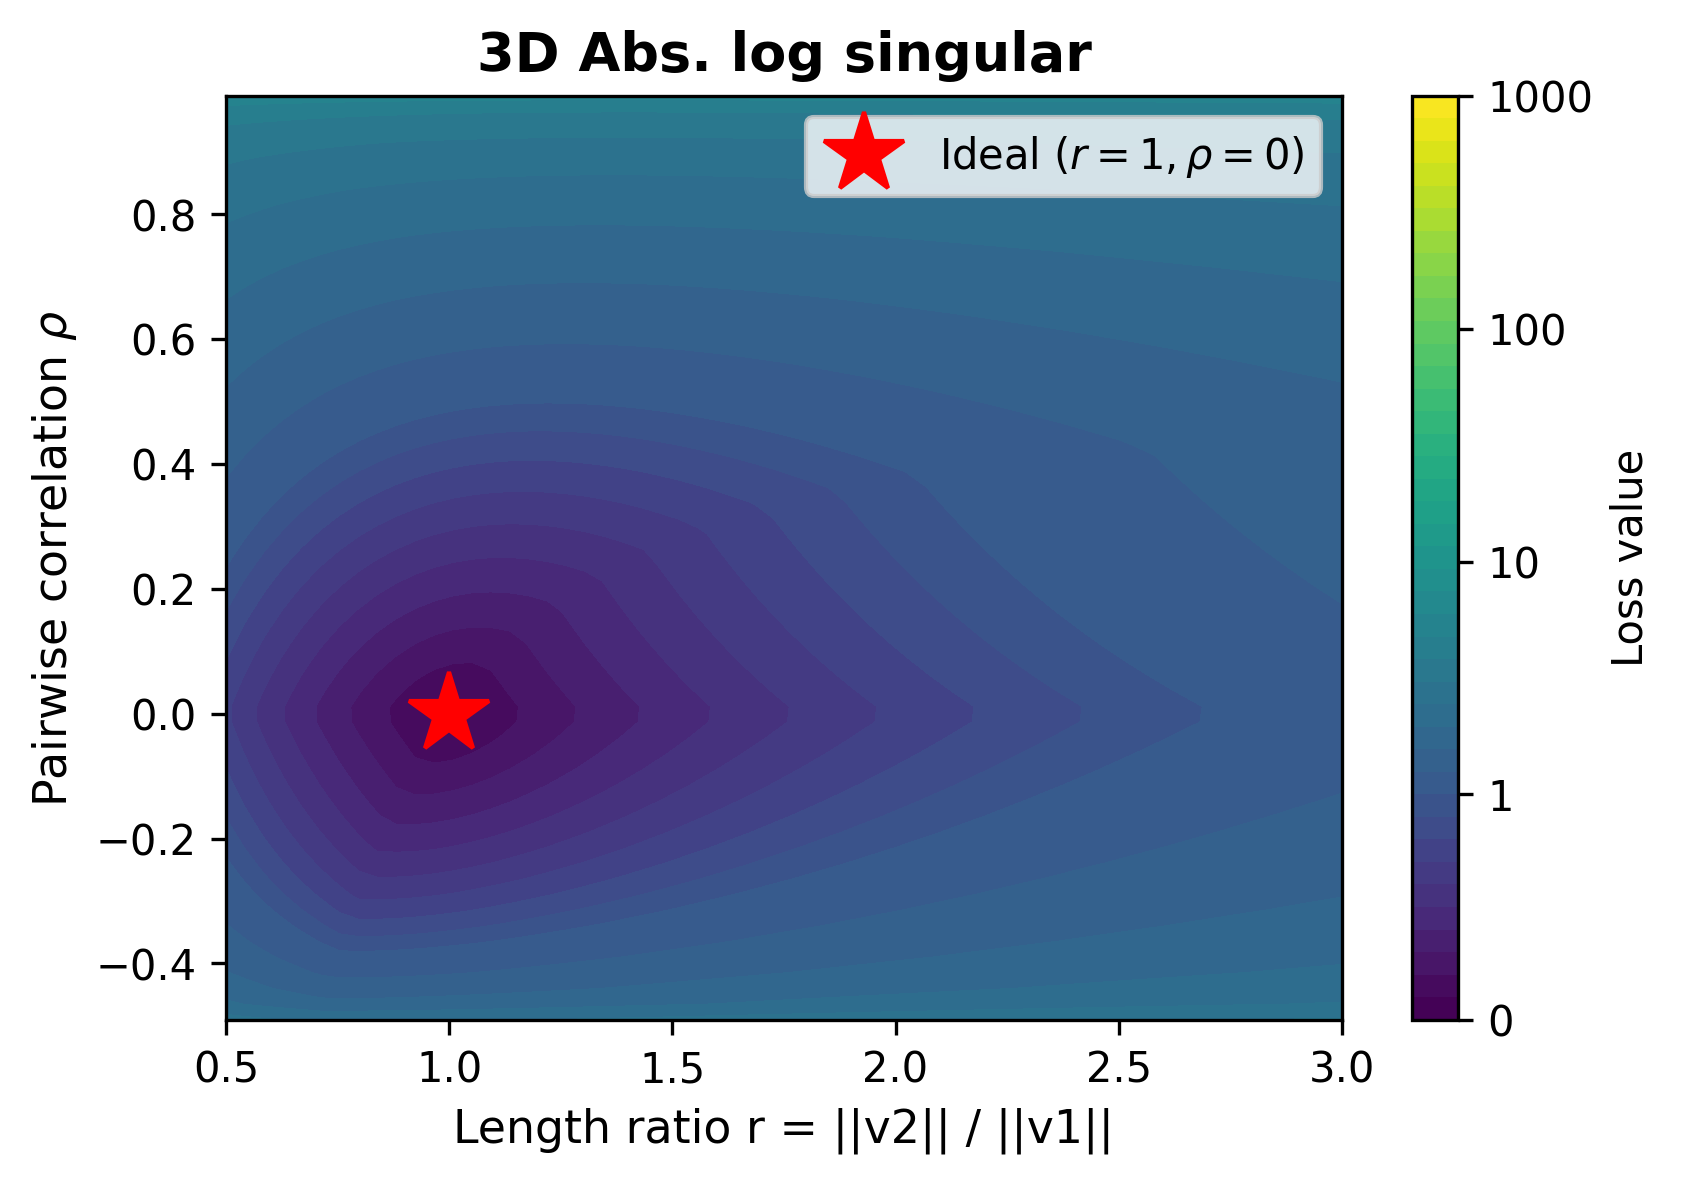
\includegraphics[width=0.48\linewidth]{../figures/loss_3d_equicorr_absolute_log_singular_values.png} &
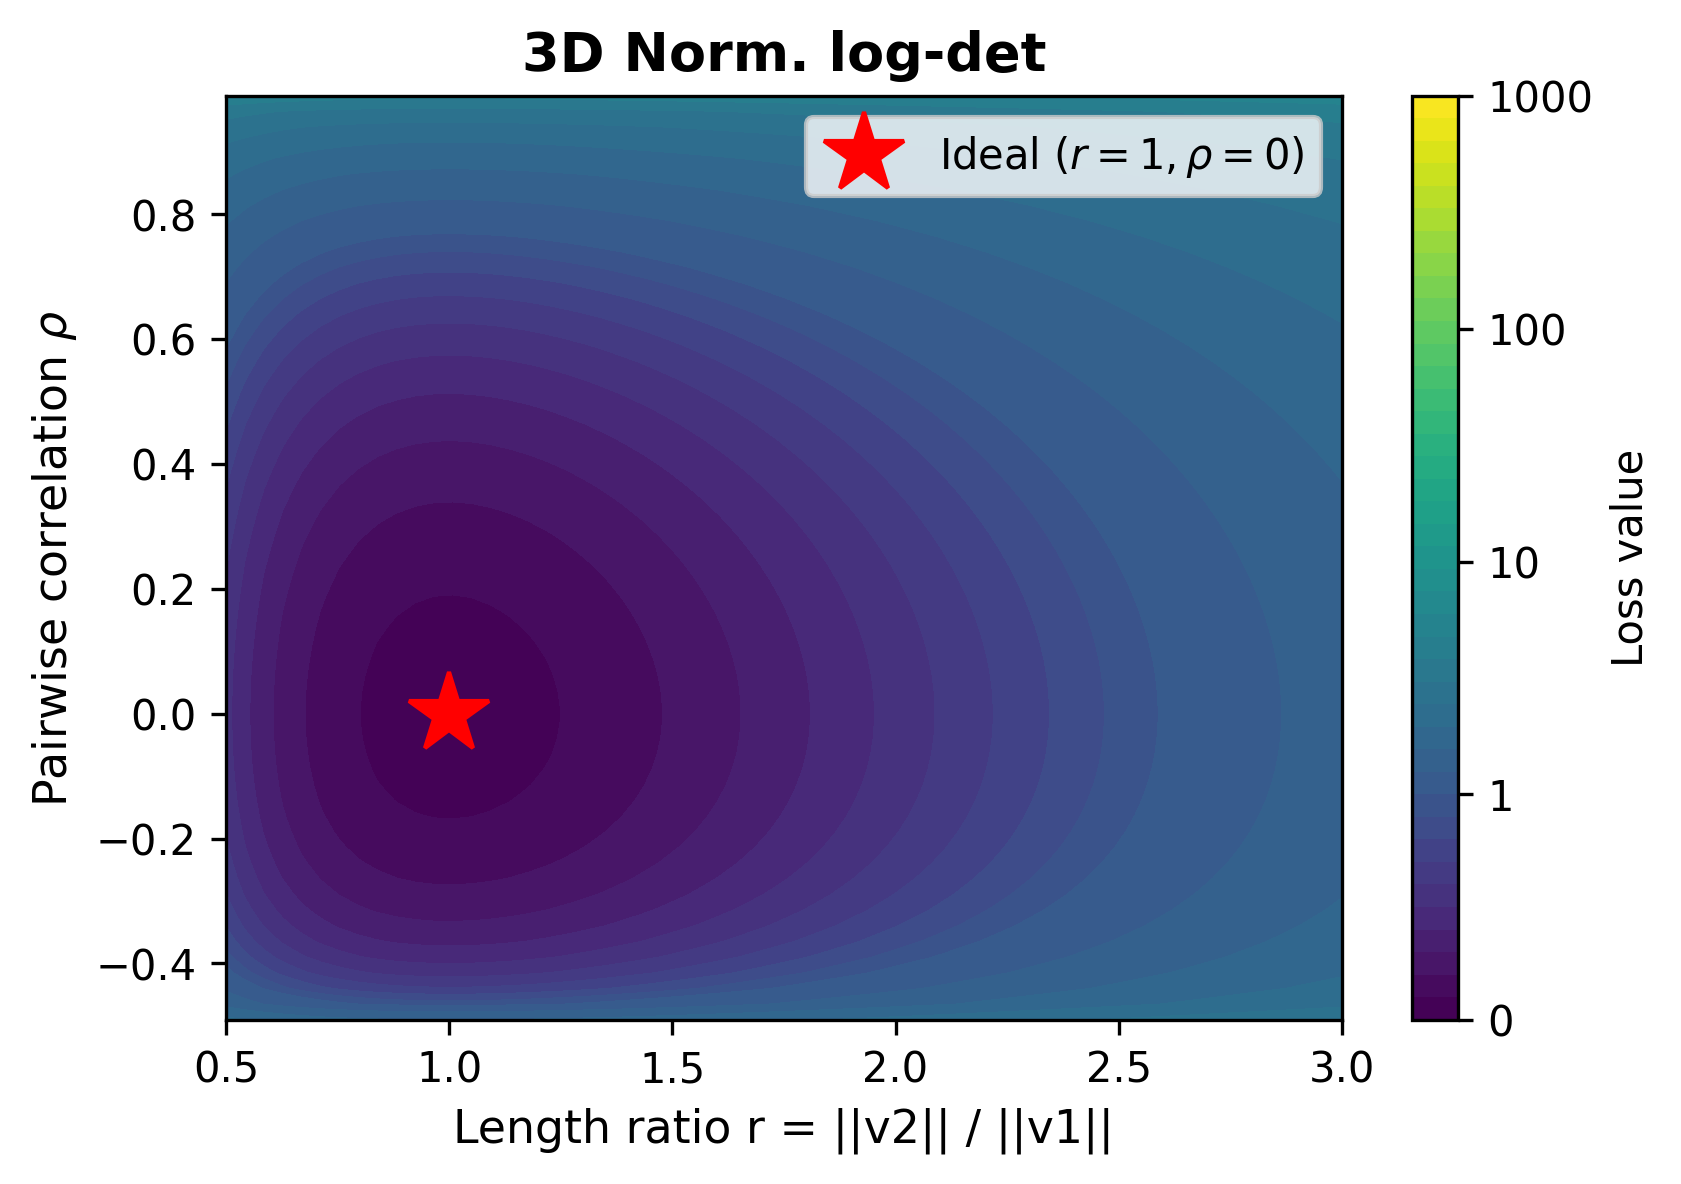
\includegraphics[width=0.48\linewidth]{../figures/loss_3d_equicorr_normalized_logdet_volume.png} \\
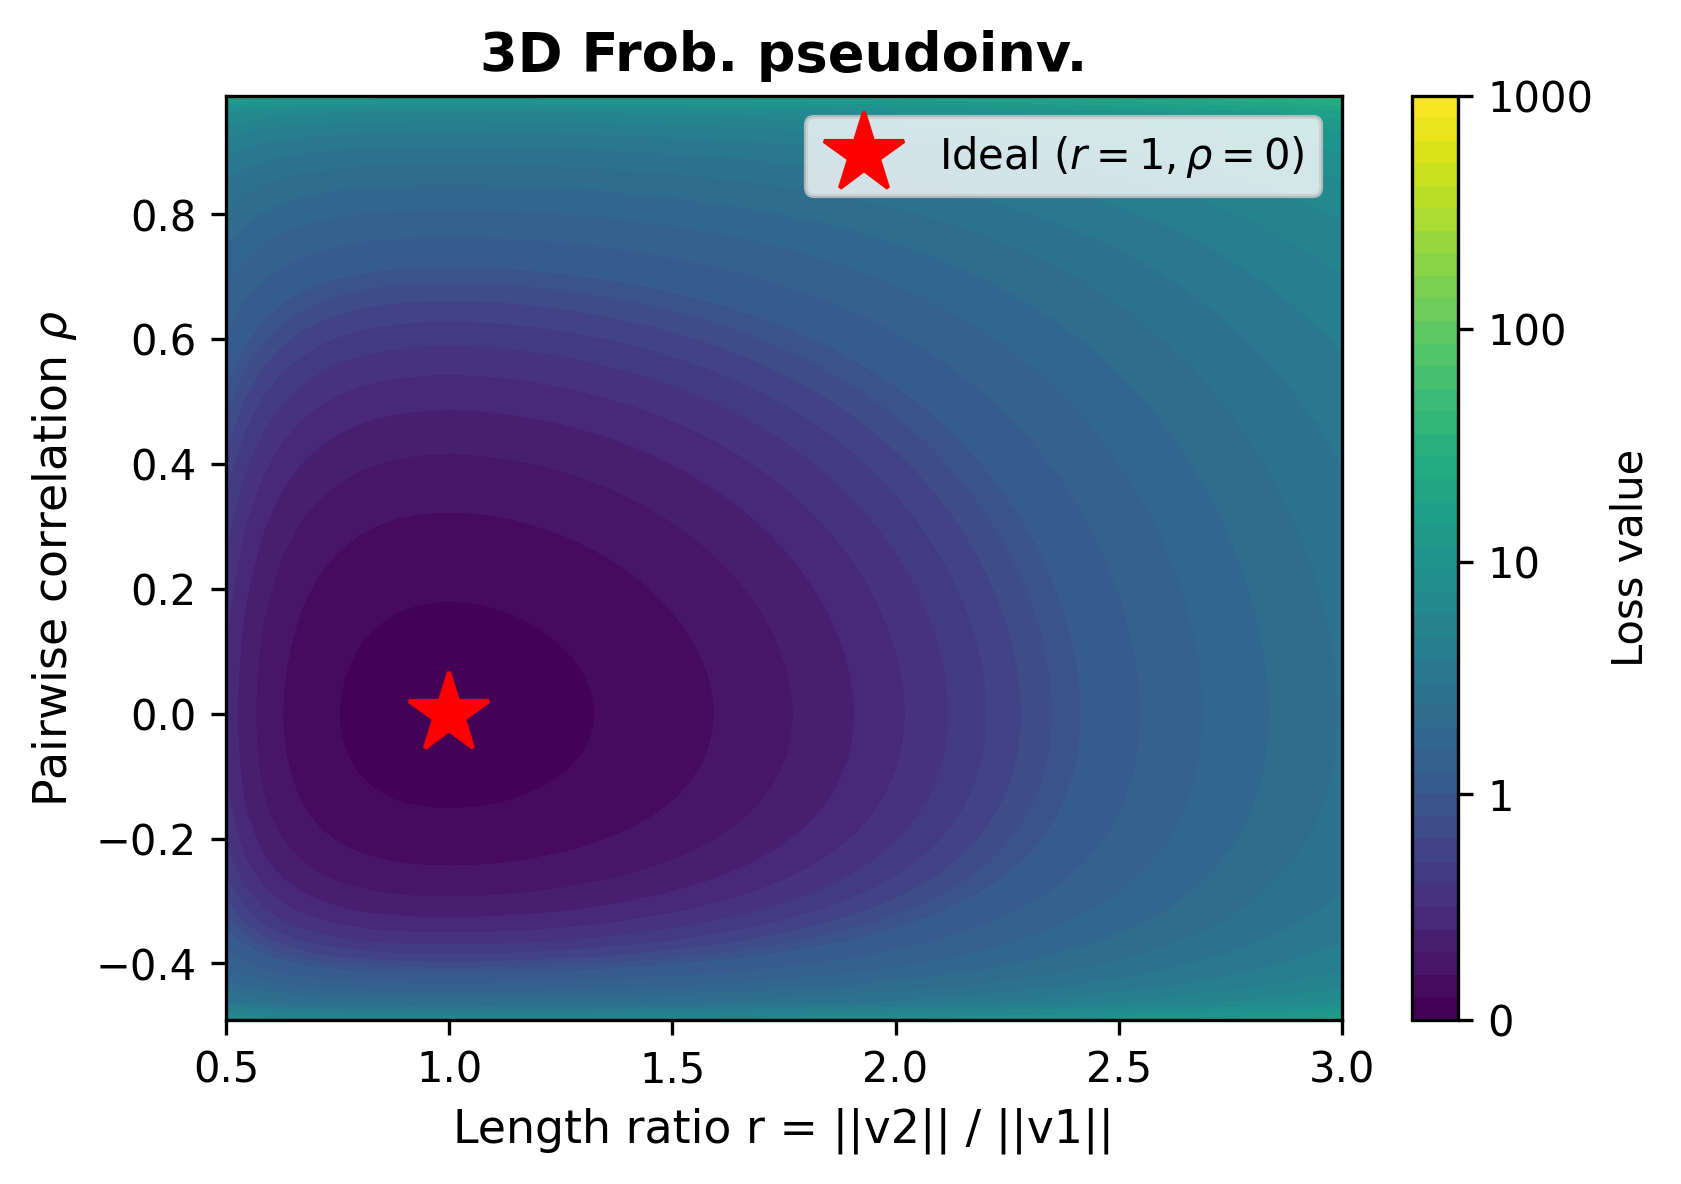
\includegraphics[width=0.48\linewidth]{../figures/loss_3d_equicorr_frob_pseudoinverse.png} &
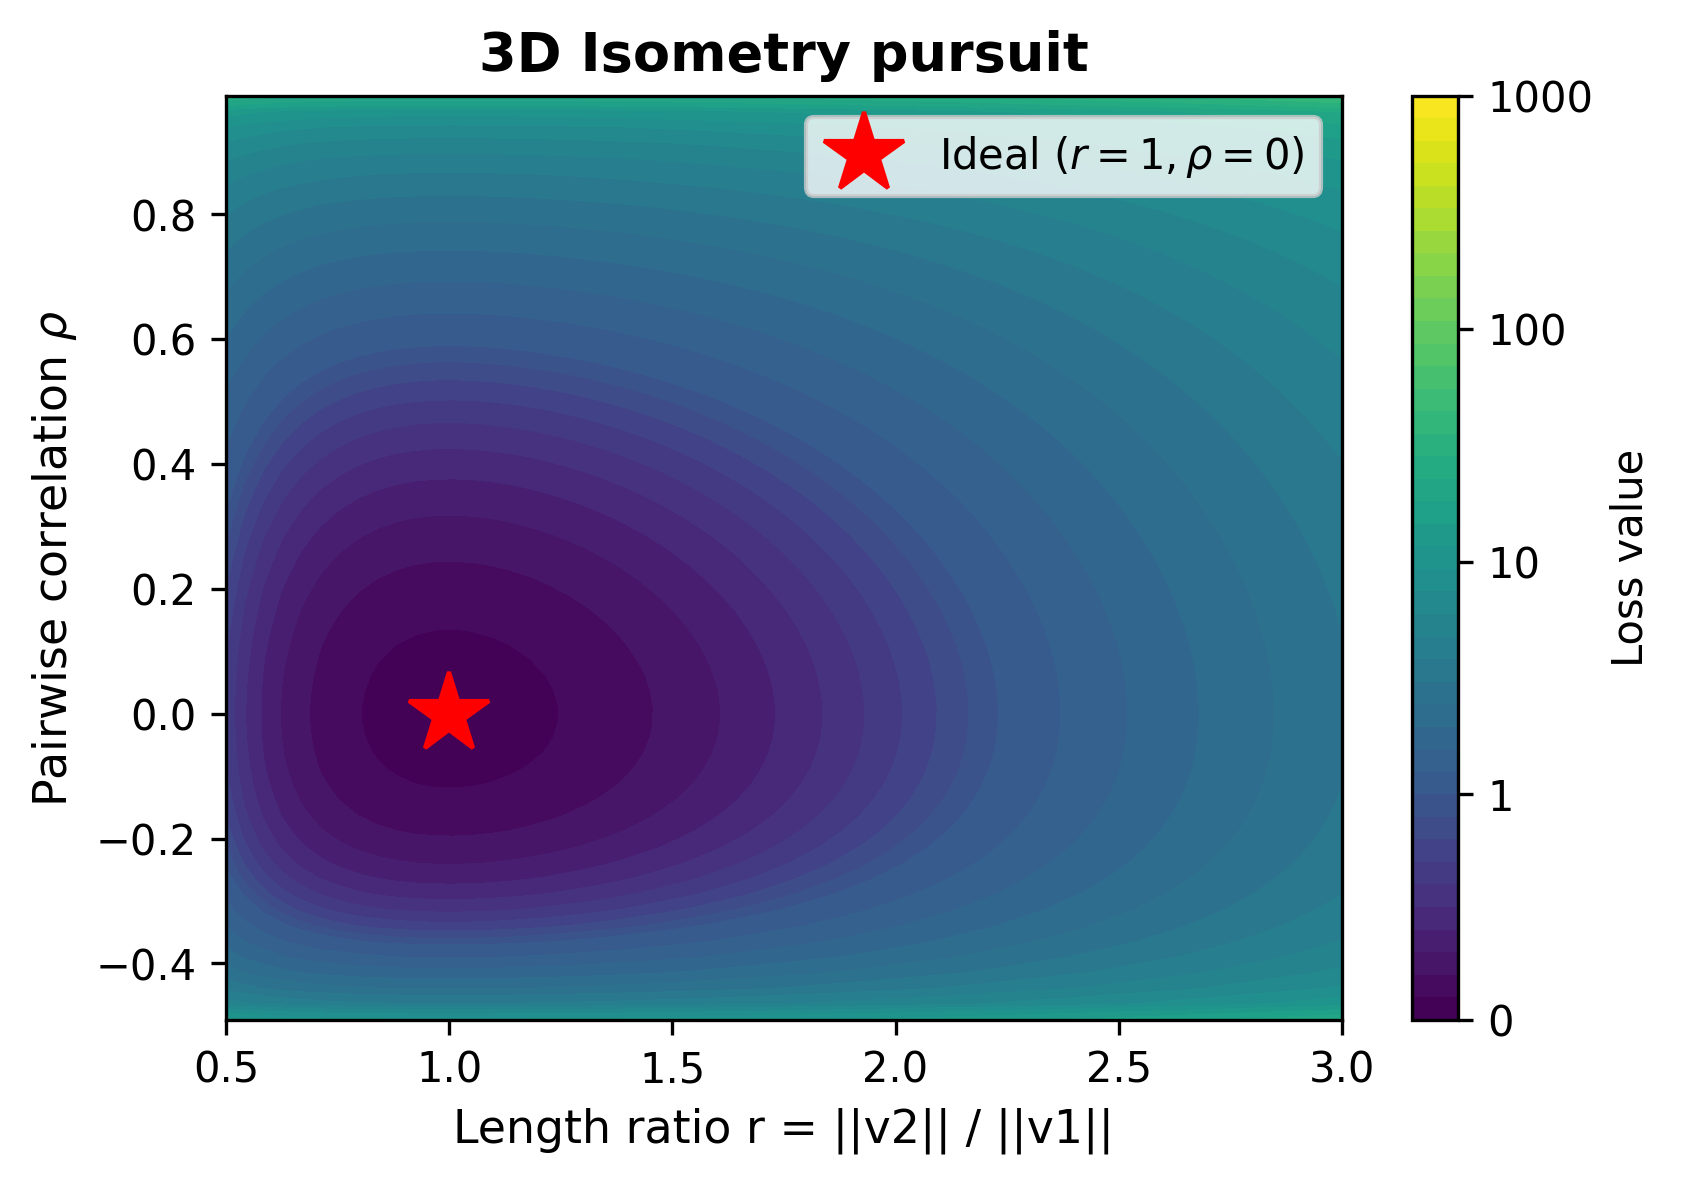
\includegraphics[width=0.48\linewidth]{../figures/loss_3d_equicorr_gl_pseudoinverse.png}
\end{tabular}
\endgroup \caption{Equicorrelated $3 \times 3$ matrices.}
\label{fig:loss_3d_equicorr_landscapes}
\end{subfigure}
\caption{Loss function comparison.
(a) Each landscape varies the length ratio $r$ and angle $\theta$ between two column vectors.
(b) Each matrix consists of three vectors in $\mathbb R^3$ with lengths $(1,r,1)$ and common pairwise correlation $\rho$; the horizontal axis varies $r=\|v_2\|_2/\|v_1\|_2$ and the vertical axis varies $\rho$.
S-divergence and absolute log singular value are representative generic spectral losses.
The red star marks the ideal orthonormal setting: $(r,\theta)=(1,\pi/2)$ in (a) and $(r,\rho)=(1,0)$ in (b).
We choose $g(t)=|\log t|$, whose spectral loss favors unit column length in the $2\times2$ family in (a), but even this choice fails in the $3\times3$ family in (b).
See Table~\ref{tab:loss_functions} for mathematical definitions.}
\label{fig:loss_comparison}
\end{figure}
